\documentclass[10pt,conference,compsocconf]{IEEEtran}

%\usepackage{times}
%\usepackage{balance}
\usepackage{url}
\usepackage{graphicx}	% For figure environment
\usepackage{xcolor}
\usepackage{booktabs}
\usepackage{framed}
\usepackage{mathtools}
\usepackage{amssymb}


\newcommand\R{\mathbb{R}}
\newcommand\todo[1]{\textcolor{red}{Todo: #1}}

\begin{document}
\title{Write-Up Robot Judge}

\author{
  Huber Simon\\
  Department of Computer Science, ETH Zurich, Switzerland
}

\maketitle

\begin{abstract}
  This semester I took the course "Building a Robot Judge: Data Science For the Law" given by Professor Ash. The course gave us an overview over tools and best practices from Natural Language Processing (NLP) and how to apply them to social topics, mainly Law and Politics. As a final project we had to reuse some of the tools learned in the lecture and apply them to a new project. For me specifically I tried to reuse Topic-Models and Neural Networks and tried to apply them to Twitter data with the idea to figure out how politicians Twitter behavior changes through the course of specific events as for example when an election happens. This Write-Up is the result of this project. 
  
\end{abstract}

\section{Introduction}
Automatic analysis of text written or said by politicians is useful in many ways. And they come in many forms - spoken on the senator floor, tweeted on Twitter and printed in papers. 
Topic models are one method to analyze such text and one of its main functions is to group documents with similar content. A lot of this techniques are unsupervised for multiple reasons: \begin{enumerate}
	\item There is not enough data that is already labeled. 
	\item The target data set is very small or very specific. 
\end{enumerate} 
But there actually is already enough data labeled for a very wide range of topics on Twitter. By interpreting hashtags as labeled data for topics we can expand the labeled data immediately. With 500 million tweets per day \cite{twitter_stats} and many of them tagged with different topics. From a sample of 1 million random tweets 15.32\% had at least 1 tag. The idea then was simple, learn a topic model through hashtags and transfer the learned model to other domains. In this work we were interested in applying it to speeches of politicians. In particular we thought about the following ideas: How does the topics of a speech for a senator change if he is up for reelection? How are the topics distributed for a democrat or for a republican senator? Can we use hash tags to predict the party? And lastly how do the topics compare between speech and Twitter for a specific politician and to the general trendy topics? \\
The paper continuous in the following manor: 
\begin{enumerate}
	\item In Section \ref{sec:Data} I describe the used datasets and how they were obtained. \\
	\item In Section \ref{sec:Plan} I discuss the two models we used to predict the hash tags and why one failed. \\
	\item In Section \ref{sec:Experiments} I describe the planned and executed experiments as well as their result.\\
	\item In Section \ref{sec:Discussion} I discuss the results.\\
	
	\item And finally In Section \ref{sec:Summary} I summarize and conclude the paper. \\
	\item The Code Section \ref{sec:Code} is more of an isolated part that describes the Github repository and what is found where. 
\end{enumerate}




\section{Data}
\label{sec:Data}
This section contains the description of the used datasets, how they were obtained and the overall statistics. 
\subsection{Twitter Data}
Twitter has a rule that one is not allowed to save tweets along with text and make it then publicly available as a dataset. This is because if one wants to make any changes to the tweets e.g. delete them etc. this is no longer globally possible if they are saved somewhere else online. So one is only allowed to save the unique ID that can be used to retrieve the tweets with the Twitter API. A website that makes many important datasets available in this manner is found in  \cite{twitter_datasets}. I downloaded two datasets.
\subsubsection{Congress Dataset}
The 115th U.S. Congress Tweet Ids dataset contains 2,041,399 tweets. It covers a date distance from 2017-01-27 to 2019-01-02. It therefore covers 1 year before the senate elections and one year after the senate elections which makes it definitely very interesting for us. The metadata of the dataset specifies the date range but there were tweets in the dataset that were back as late as 2012. 
\subsubsection{News Dataset}
The News Outlet Tweet Ids downloaded is a fallback dataset which in case the congress dataset was to "fuzzy" could be used to train on more well written, structured and diverse topic distributed dataset. Which was of course just an hopeful assumption backed by the assumption that journalists were more careful when crafting tweets (e.g. by not using slang and slurs). I ended up not using this dataset. 
\subsection{Speeches Data}
The congressional records and therefore the speeches can all be publicly accessed on the congress page \cite{congress_page}. But this side makes it very hard to access and download specific information. So people developed software packages that parse this side for the information and presents it in an accessible format mostly json. I first tried a package from another student but due to some bugs for my specific use case I had to switched to \cite{congress-downloader} which worked very nicely. I used it to parse and save all speeches given in the years 2017 and 2018.


\section{Plan}
\label{sec:Plan}
In the first part of this Section I will tell about LDA and about how I planed to adapt LDA so it is able to predict hashtags. In the second part I give a summary of the neural network based method that finally worked for predicting hash tags. 
\subsection{Latent Dirichlet Allocation (LDA)}
\subsubsection{Standard LDA}
LDA was one of the algorithms for topic models that got presented in class. The generative model to generate a word makes it very simple to think about LDA. Given a document sample a topic and for this topic sample a word. And the word which is observed is used to learn the corresponding distributions. \\
\textbf{More formally} the process depicted in Figure \ref{fig:ldaplate} is defined as: 

\small
\begin{align*}
&\textit{Given } \alpha, \beta \\
&\textit{Sample topic-distribution: } \theta_m \sim Dir(\alpha)\\
&\textit{Sample word-in-topic-distribution: } \phi_k \sim Dir(\beta) \\
&\textit{Sample word-topic from topic-distribution: } z_{mn} \sim Cat(\theta_m) \\
&\textit{Sample word from word-in-topic-distribution: } w_{mn} \sim Cat(\phi[z_{mn}])
\end{align*}
\normalsize
Where $\alpha \in \R^K, \beta \in \R^{|V|}$ are the parameters for the dirichlet distribution. 

\begin{figure}
	\centering
	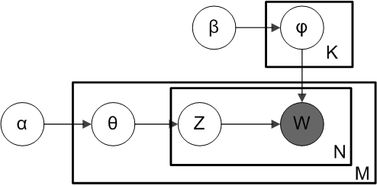
\includegraphics[width=0.7\linewidth]{images/lda_plate}
	\caption{Plate notation for LDA with Dirichlet distributed topic-word distributions.}
	\label{fig:ldaplate}
\end{figure}


\subsubsection{Extended LDA}
So naturally I thought it should be simple to extend LDA so that it can also predict hash tags in the following way. For some document and its document-topic distribution I sample two topics and then for the topic-word distribution I sample a word and additionally to the topic-word distribution I just have a topic-hashtag distribution from which I sample a hashtag. And the we can learn the correct distributions since we observe both word and hashtag. \textbf{More formally} we have only 3 additions (inserted in blue) to the process as defined in normal lda: 

\small
\begin{align*}
&\textit{Given } \alpha, \beta, \gamma \\
&\textit{Sample topic-distribution: } \theta_m \sim Dir(\alpha)\\
&\textit{Sample word-in-topic-distribution: } \phi_k \sim Dir(\beta) \\
& \textcolor{blue}{\textit{Sample hashtag-in-topic-distribution: }} \kappa_k \sim Dir(\gamma) \\
&\textit{Sample word-topic from topic-distribution: } z^{(w)}_{mn} \sim Cat(\theta_m) \\
&\textit{Sample word from word-in-topic-distribution: } w_{mn} \sim Cat(\phi[z_{mn}])\\
&\textcolor{blue}{\textit{Hashtag-topic from topic-distribution: }} z^{(t)}_{mt} \sim Cat(\theta_m) \\
&\textcolor{blue}{\textit{Hashtag from hashtag-in-topic-distribution: }} t_{mn} \sim Cat(\kappa[z_{mn}])\\
\end{align*}
\normalsize
Where $\alpha \in \R^K, \beta \in \R^{|V|}, \gamma \in \R^K$ are the parameters for the dirichlet distribution. The plate in Figure \ref{fig:ldaplate2} depicts the whole process graphically.
\begin{figure}
	\centering
	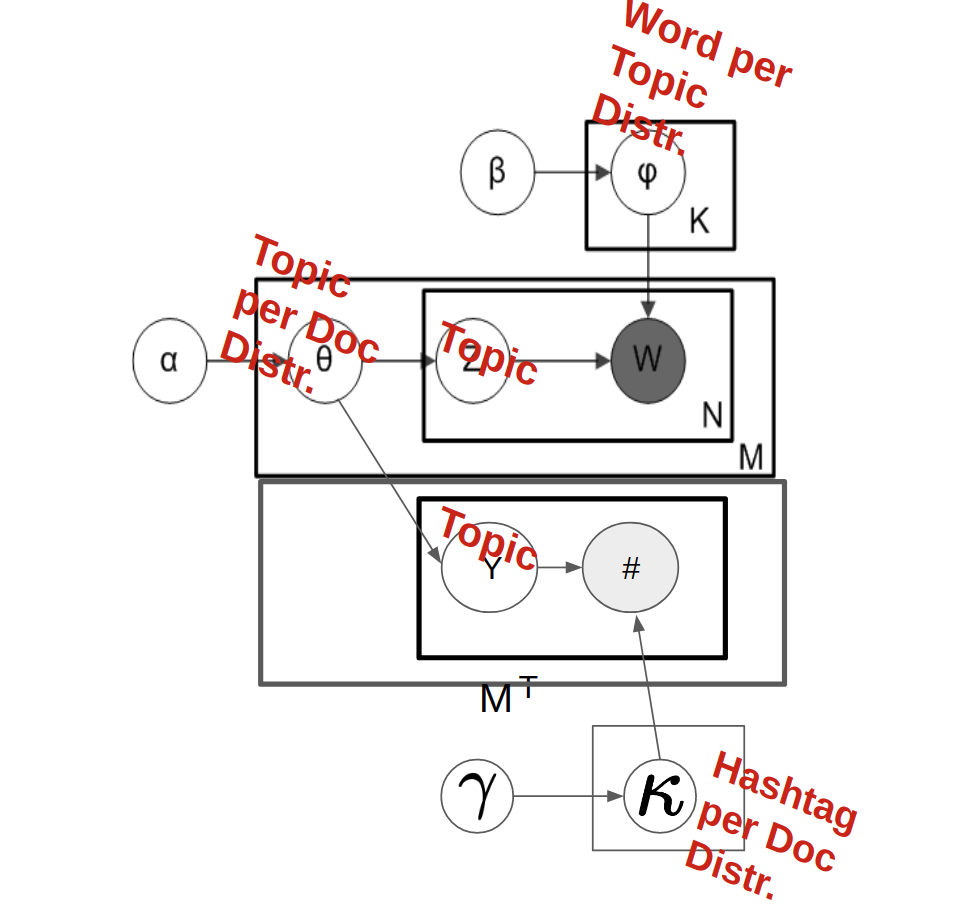
\includegraphics[width=0.7\linewidth]{images/extended_lda}
	\caption{Plate diagram of extended version of LDA with additional distribution for hashtags for a given topic. }
	\label{fig:ldaplate2}
\end{figure}

\subsection{Training}
Now the generative model is only the first step because we're not interested in generating words. We're interested in the so called posteriori distribution: Given words what are the topic-distribution of a document. Then from that generate hashtags by sampling a topic and sampling a hashtag for the document. This means that we have a so called inference problem and normally one applies bayes formula to get the topic distribution: \[ p(\theta_m | w) = \frac{p(w | \theta_m)p(\theta_m)}{p(w)} \] But the so called evidence term \[p(w) = \int_{\theta_m} p(w | \theta_m)p(\theta_m) d\theta_m^K \] is very hard to compute because every new possible topic increases computing time exponentially so this is nearly impossible to compute already for very little amount of topics. 
Researchers have proposed different methods to approximate this posteriori distribution with other methods and there are a lot of software frameworks that automatically calculate the posterior distirbution. I decided to use pyro \cite{bingham2018pyro} which allows to describe the generative model in a very pytonian way and uses pyTorch \cite{paszke2017automatic} as backend for matrix and optimization calculations which should make it ideal for big datasets. See the Code Section \ref{sec:Code} for an overview of what is implemented in which files.   The optimization process is either via a monte carlo method (MCMC) or via Variational Inference (VI). Bot methods are explained in the next two subsections very briefly. 

\subsubsection{Variational Inference}
The big idea in Variational Inference (VI) is to propose a proposal distribution $q_\lambda(\theta_m)$ which gets adapted via parameter $\lambda$ to be as close as possible to the real distribution we care about $p(\theta_m | w)$. Closeness is measured via kullback-leibler divergence but this can't be calculated directly most of the time so alternatively one maximizes the so called ELBO which minimizes the kullback-leibler divergence. 
\[ ELBO = \mathbb{E}_{q_\lambda(\theta_m)} [log p(\theta_m, w) - log q_{\lambda}(\theta_m)] \]
Then to maximize the ELBO in most software packages one calculates the gradient and applies one of the nowaways many optimization algorithms. (Adam, RMSprop, SGD, etc.)\\
Since I used pyro to implement this, in pyro $q_\lambda$ is described in the so called "guide" function and the joint distribution $p(\theta_m, w)$ is described in the so called "model". 

\subsubsection{Markov Chain Monte Carlo}
Markov Chain Monte Carlo (MCMC) algorithms are a bit more involved in theory and there are a lot more flavors then in variational inference. But the underlying idea is quite similar to VI. MCMC algorithms propose a markov chain from which they draw correlated samples when moving from state to state in this chain but which promises to converge to the correct distribution. Now one may ask why we do not use this all the time when it converges to the correct distribution? Sadly such a chain has a so called "warm up" stage where we have to throw away samples up to the point where the distribution is burned it and we do not know how long this warm up phase is. Therefore normally one uses empirically defined rules and tests to estimate the length of the warm-up phase. A second problem is that complicated distributions get broken up into multiple conditional distributions and it can get slow to sample such distributions sequentially. \\

\subsection{Tweet2vec - Recurrent Neural Network}
After the extended LDA somewhat failed I read multiple papers and tested a multitude of other models. The one that finally worked was a neural network based solution: Tweet2Vec \cite{DhingraZFMC16}. The basic idea behind this model is that they view the character as smallest unit rather then the word as in LDA. This brings quite a few advantage. Most importantly misspelled words, slangs and slurs can be encoded with the same embedding meaning much easier. And we do not have to save all the words which due to the many abbreviations and slangs on Twitter can blow up the vocabulary very much. In the congress dataset we have 11'498'020 number of different tokens. Furthermore they assume that a tweet has some latent representation/embedding and from this latent representation/embedding they predict the hashtag. To get a loss they use cross entropy loss based on predicted hashtag versus given hashtag. The neural network is mainly built out of Bi-directional Gated Recurrent Unit (Bi-GRU) which behave similarly as LSTM's (Long short-term memory) blocks. The size of the input is reasonable constraint on the number of characters a tweet can have - 145. The embedding part of the tweet2vec neural network can be seen in Figure \ref{fig:tweet2vecembedding}. The decoder part is just a dense layer with the number of neurons equal to the number of hashtags. The output of this dense layer is then used as input for the softmax function to get the probability of each hashtag. 
\begin{figure}
	\centering
	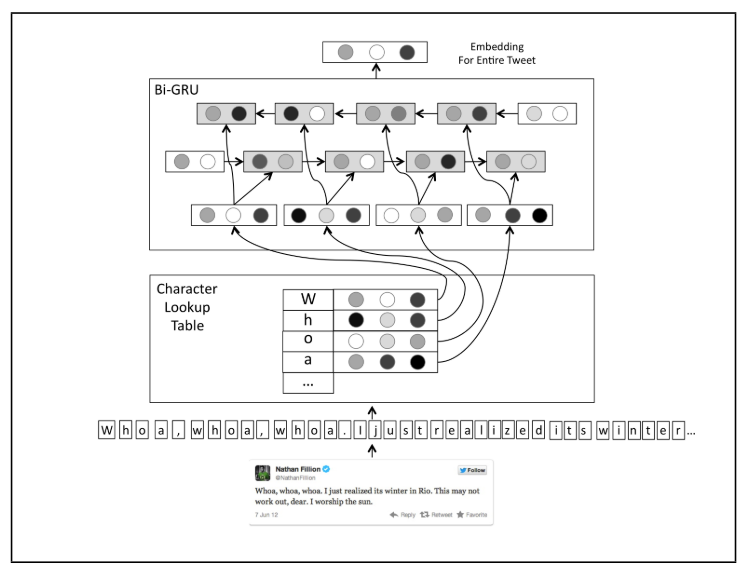
\includegraphics[width=0.7\linewidth]{images/tweet2vec_embedding}
	\caption{Tweet2vec embedding part of the neural network. The source is the original paper \cite{DhingraZFMC16}}.
	\label{fig:tweet2vecembedding}
\end{figure}


\begin{table}[]
	\centering
	\begin{tabular}{@{}lll@{}}
		\toprule
		Name       & Party      & Num. Speeches \\ \midrule
		Feinstein  & D   &       2        \\
		Stabenow   & D   &       1        \\
		Klobuchar  & D   &     1          \\
		Menendez   & D   &     1          \\
		Cantwell   & D   &      1         \\
		Warren     & D   &   1            \\
		Gillibrand & D   &        1       \\
		Tester     & D   &     1          \\
		Manchin    & D   &      1         \\
		Murphy     & D   &     5          \\
		Baldwin    & D   &       1        \\
		Hirono     & D   &        1       \\
		Carper     & D   &      1         \\
		Sanders    & I   &      1         \\
		Kaine      & D   &         1      \\
		Brown      & D   &      3         \\
		Heinrich   & D   &       1        \\
		Whitehouse & D   &     1          \\
		Casey      & D   &     1          \\
		Wicker     & R &         0      \\
		Barrasso   & R &    2           \\
		Fischer    & R &         1      \\
		Cruz       & R &      2         \\
		King       & I &     3          \\ \bottomrule
	\end{tabular}
	\caption{List of senators up for reelection in 2018. (D = Democrat, R = Republican, I = Independent).}
	\label{tbl:senators}
\end{table}


\section{Experiments \& Results}
\label{sec:Experiments}
First lets reiterate more concrete about what we want to figure out and then subsequently how we design the experiments to test our hypothesis. 
We start with a simple one: Can we tag speeches of politicians with hashtags learned from twitter? Then we go on to figure out how tags compare for someone giving a speech before and after campaigning for reelection. 

\subsection{Can we tag speeches of politicians with hashtags learned from twitter? }
\subsubsection{Data}
The politician set consisted of 449334 tweets which we splitted randomly into 90\% training data and 10\% testing data. I counted all the hashtags and removed all that were not in the top 500 used hashtags (from 39671 total). The 500 had no specific reason other then to simplify the prediction and that there are a lot of tags that are used very few times which makes it not relevant for my use case. 

\subsubsection{Results}

As explained in previous sections I used tweet2vec.  In Figure \ref{fig:tweet2vectraining} one can see that we got nearly 25\% recall for tag number 1 which is quite good considering how difficult the task is (Randomly predicting one of the top 500 would result in 0.2\% recall). For the speeches I was only interested in the senators up for re-election. It is a set of 24 senators listed in Table \ref{tbl:senators} with their corresponding party and the number of speeches they gave in the years 2017 and 2018. \\
Sadly and for me quite unexpected this dataset of speeches is very small.  But it does not hinder us to tag the available speeches. To tweet2vec to be able to work on the speeches I had to cut it up into pieces of 145 and additionally I did some preprocessing like stemming, removing stop words and removing line breaks just to get a bit shorter speeches and get more content into those 145 characters. 

In the boxes one can see the input for the trained tweet2vec in the top part and the tags tweet2vec predicted in the bottom part. 

\begin{framed}
	\textbf{Senator Sanders}: \\
	support vote pension issue million american worker percent pension promise government allow happen stand worker meeting earlier today dealing \\
	Tags: Kavanaugh WhatAreTheyHiding NM UK IIOA
\end{framed}
\begin{framed}
	\textbf{Senator Cruz}: \\
 president authority refuse enforce president obama decree would enforce federal immigration exactly virtually every republican denounce executiv
 \\
	Tags: ACA healthcare NM ClimateAction ProtectOurCare
\end{framed}

From just checking the speeches vs the tags by hand it does not seem to be very effective in predicting tags for speeches. 
I really tried to also find a positive example but I just couldn't really find a satisfying one.

 
\subsection{How does being before an election affect the tags a politican uses? }
After wasting a lot of time on the tagging speeches part I concentrated the little rest of my time on only analyzing the raw Twitter data. And one can say that for some senators definitely tweets differently and is affected when having an election. I picked a democratic senator and a republican senator to showcase how tweets change. Local topic get very important for senators and most tweets will get tagged with the state their from. In figure \ref{fig:hironobeforeafterelection} its the case for the 2012 election where Senator Hirono wants to get elected for Hawaii. In Figure \ref{fig:senatorfischerbeforeafterelection} one can see the number of tweets at a specific date from Senator Fisher of the republicans. It shows that shortly before the election in Nebraska, Nebraska specific tweets definitely spiked.\\
But it is definitely not an if and only if deduction. There are a lot of Senators who don't care about tweeting for local problems e.g. Senator Warren and Senator Sanders. See Figure \ref{fig:tweetsSanders} for the distribution of tags for Senator Sanders and \ref{fig:tweetsWarren} for the distribution of tags over time for Senator Warren. In both it is obvious that they have more global priorities then their own states. The plots for all the other Senators can be checked in my github repository see Section \ref{sec:Code}. But not only could it be that the tweet behaviour does not change but that a Senator could start tweeting about local events with no local election coming up. An example for this is Senator Cruz who had a hard election in Texas. But in the year of the election there was also a hurrican as strong as all 10 years and he tweeted a lot about that in that same time frame which is also the time of the election seen in Figure \ref{fig:senatorcruztop5tweetsmid20172018}.
 
\begin{figure}
	\centering
	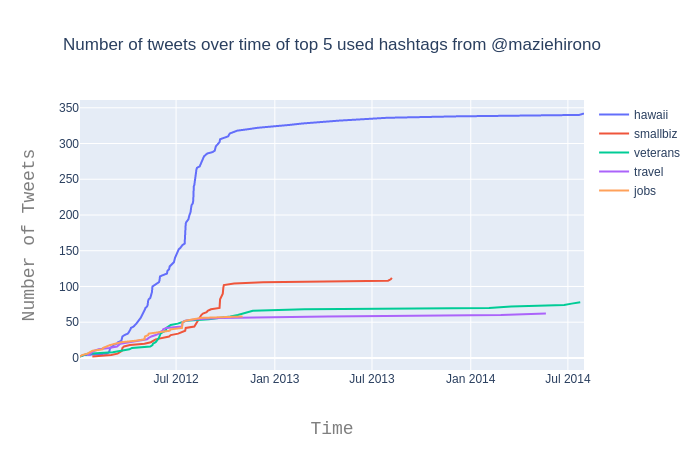
\includegraphics[width=0.7\linewidth]{images/hirono_before_after_election}
	\caption{Cumulative sum of top 5 topics of senator Hirono from Hawaii. }
	\label{fig:hironobeforeafterelection}
\end{figure}


\begin{figure}
	\centering
	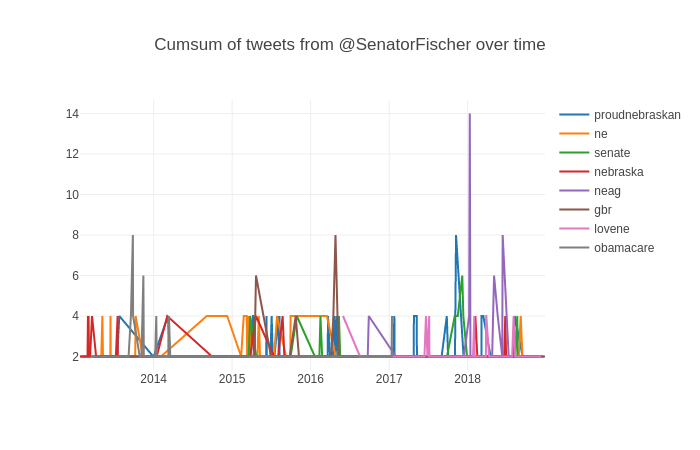
\includegraphics[width=0.7\linewidth]{images/senator_fischer_before_after_election}
	\caption{Senator Fischer from Nebraska number of tweets from 2012 - 2019 counted at specific points in time. Only tweets counted with tags of top 8 tags. \#ne = nebraska, \#neag = nebraska agrar, \#lovene = love nebraska.   }
	\label{fig:senatorfischerbeforeafterelection}
\end{figure}
\begin{figure}
	\centering
	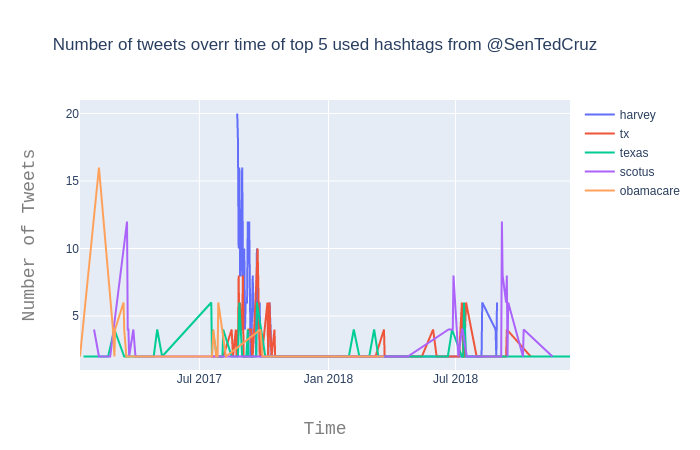
\includegraphics[width=0.7\linewidth]{images/senator_cruz_top5_tweets_mid2017_2018}
	\caption{Senator Cruz from Texas top 5 used tags tweets distribution from mid 2017 to end 2018.}
	\label{fig:senatorcruztop5tweetsmid20172018}
\end{figure}

\begin{figure}
	\centering
	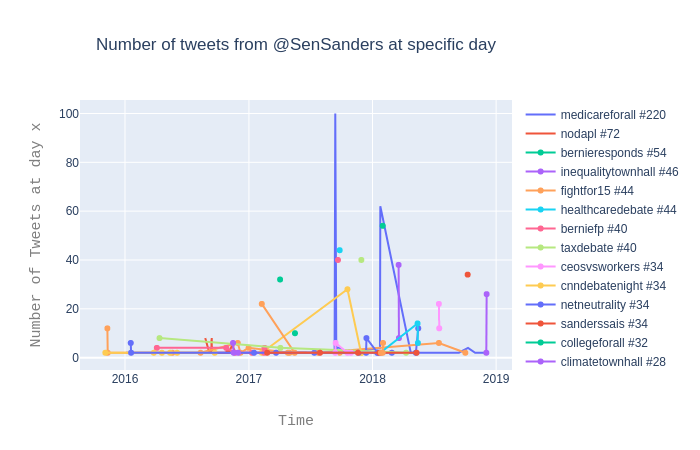
\includegraphics[width=0.7\linewidth]{images/tweets_of_sensanders_overtime}
	\caption{Number of tweets of senator Sanders at a specific day.}
	\label{fig:tweetsSanders}
\end{figure}
\begin{figure}
	\centering
	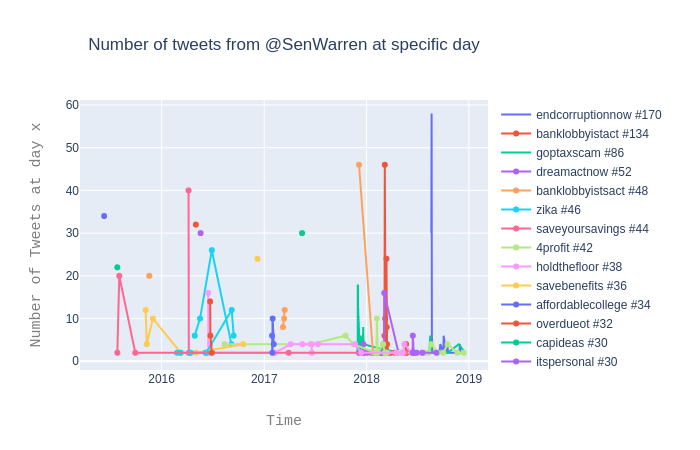
\includegraphics[width=0.7\linewidth]{images/tweets_of_senwarren_overtime}
	\caption{Number of tweets of senator Warren at a specific day.}
	\label{fig:tweetsWarren}
\end{figure}

\begin{figure}
	\centering
	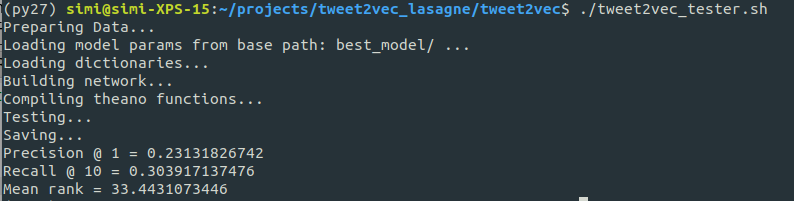
\includegraphics[width=0.7\linewidth]{images/tweet2vec_training}
	\caption{Results for testing on validation set. (10\% of original dataset).}
	\label{fig:tweet2vectraining}
\end{figure}

\section{Negative Results}

LDA with Pyro just didn't work. I tried a multitude of different proposal distributions and even neural networks. It just didn't really converge nicely. I initially thought that the problem was my extension on top of LDA. But it didn't work for LDA aswell. So that comparison is simpler I directly make boxes in the text that shows the result without having an extra Figure with the results in it. 

\subsection{Sklearn News Dataset}

Since in the lecture we learned about sklearn I thought to test the LDA implementation first with the LDA implementation from Sklearn and since Sklearn uses a provided News dataset in its examples I reused that to test my LDA pyro implementation. But first the topics I obtained with normal \textbf{LDA-Sklearn}: 
\begin{framed}
	Topic 0:\\
	law jesus christ god faith\\
	Topic 1:\\
	course training applications esa data\\
	Topic 2:\\
	card drive game remove board\\
	Topic 3:\\
	good federal new coach defense\\
	Topic 4:\\
	team players edu nhl teams\\
	Topic 5:\\
	israeli human jews israel rights\\
	Topic 6:\\
	cx c\_ ah ck 34u\\
	Topic 7:\\
	weapon models mouse copy ibm\\
	Topic 8:\\
	don just use like time\\
	Topic 9:\\
	gun right guns president new\\
\end{framed}
It definitely finds some words that belong to the same topic.\\
Then next \textbf{my Pyro-LDA} implementation:

\begin{framed}
	---- topic 0 ----- \\ 
	'would', 'attack', 'n        ', 'think', 'input', 'right', 'plaintext', 'cards'\\
	---- topic 1 -----\\
	'would', 'n    ', 'forgery', 'cryptosystem', 'provide', 'thing', 'think', 'system', 'seem', 'suppose'\\
	---- topic 2 -----\\
	'would', 'people', 'think', 'month', 'windows', 'support', 'information', 'right', 'advice', 'attack'\\
	---- topic 3 -----\\
	'would', 'right', 'n        ', 'technology', 'people', 'could', 'point', 'attack', 'wretched', 'computer'\\
	---- topic 4 -----\\
	'would', 'program', 'reward', 'case', 'right', 'windows'
\end{framed}
 And one can see that it defintly finds some words that belong together but it seems that it can't really find a hard border between the topics. Then I googled a bit about what may be could be wrong with my model and I stumbled upon an implementation provided by Pyro itself. This implementation uses a neural network as a proposal distribution for the topics. So that the neural network could find some non linear mapping between the input words to the specific topic. So I tested this as well \textbf{Pyro-LDA}:
 \begin{framed}
 	---- topic 0 -----\\
 	'anyone', 'would', 'post', 'looking', 'system', 'first', 'please', 'hello', 'article', 'several'\\
 	---- topic 1 -----\\
 	'think', 'people', 'anyone', 'could', 'would', 'please', 'interest', 'looking', 'believe', 'point'\\
 	---- topic 2 -----\\
 	'would', 'people', 'could', 'anyone', 'think', 'please', 'someone', 'try', 'believe', 'thought'\\
 	---- topic 3 -----\\
 	'could', 'people', 'someone', 'following', 'would', 'windows', 'try', 'drive', 'really', 'right'\\
 	---- topic 4 -----\\
 	'think', 'would', 'people', 'could', 'someone', 'anyone', 'question', 'drive', 'article', 'believe'
 	\end{framed} 
And it seems to have a very similar problem to my own implementation as to be able to split the result into multiple topics and not return randomly one of the top K used words.

\subsection{Results on Twitter Data}
So naturally when one is very convinced that the model should actually work and its probably the data's fault I tried my extended versions of LDA on the Twitter data anyway. And sadly it failed as well. 
\textbf{Extended Pyro - LDA - implementation Figure \ref{fig:resultldaontwitter}:}
\begin{figure}[h]
	\centering
	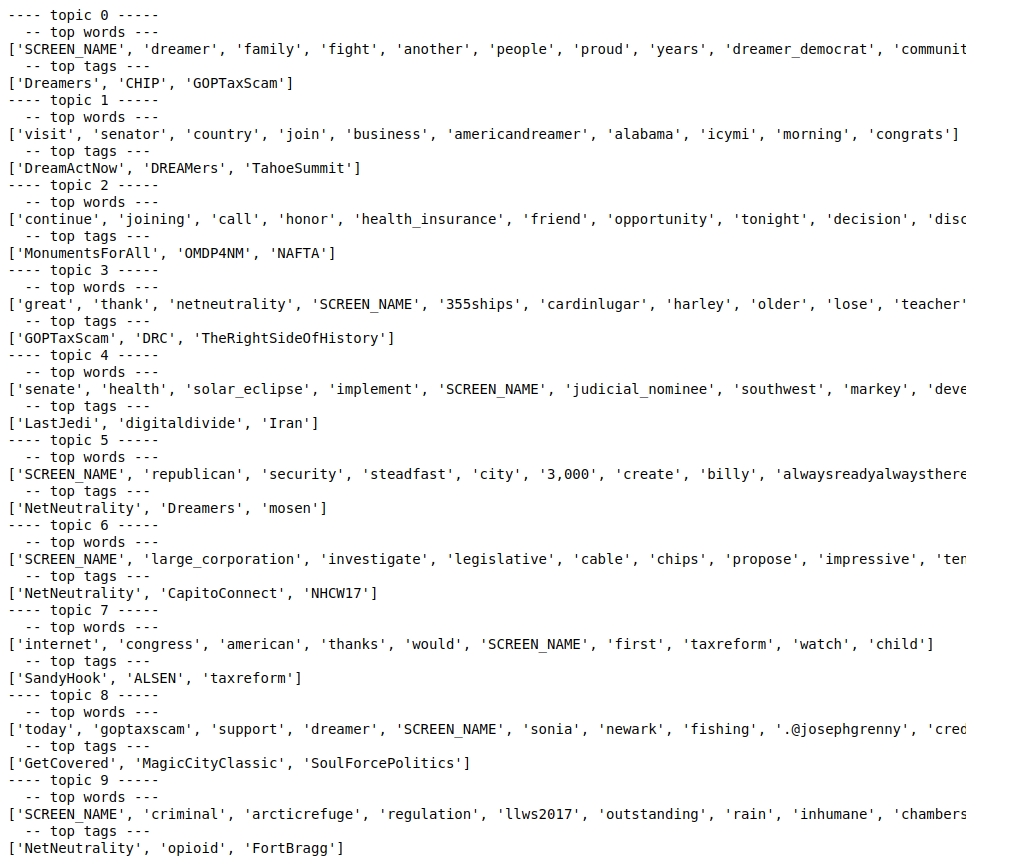
\includegraphics[width=0.7\linewidth]{images/result_lda_on_twitter}
	\caption{Results of predicting topics and hashtags together. Source: pyro\_lda\_final.ipynb}
	\label{fig:resultldaontwitter}
\end{figure}
And one can see that it has multiple tags from this 39671 that it really likes but it just can't get it to split between the topics. 



\section{Discussion}
\label{sec:Discussion}

\subsection{Data discussion}

I was quite surprised about the very small amount of speeches politicians gave on the senate floor. I think I got surprised because the media implies through extensive coverage of politicians nearly every day that there happens actually much more then actually happens. The amount of speeches makes more sense when considering that there are 100 Senators and only 148 legislative days on average per year over the last 10 years.  \\


\subsection{Lessons learned}
I want to write down a few words about the lessons I've learned and reflect a bit so that I can take something to my next project besides the technical. 
\begin{enumerate}
	\item The biggest point for me is apply the right tool to the right problem. Since I've read and heard the first time about probabilistic programming languages I searched for a way to apply it somewhere during my studies. I'm more on the graphics side in my computer science studies which made it difficult to apply it anywhere there. So along came this topic model problem and I tried everything to apply it to this problem. I think this gave me kind of a tunnel vision which lead to ignoring maybe more applicable paths.
	\item Twitter data is hard. This is definitely something I had not considered before. Due to the length restrictions on a tweet many properties that emerged from Twitter are not simple to generalize to other texts. 
	\item When working with big data probably nothing comes close to deep learning currently. I always had the urge to not use the tools that everyone else is using which punished me hard on this task because all the state of the art in this kind of area ( text / speech / vision) is based on neural networks. 
\end{enumerate}
So really in summary of this lessons: I should just be more conscious about my own biases I bring to a project and should myself ask earlier if I'm still on the right path. 


\section{Summary}
\label{sec:Summary}
In this work I tried to learn multiple models on how to predict hashtags for tweets. When correctly learned to predict tags for tweets I tried to transfer the tagging to speeches of politicians and answer some questions about how their behavior changes when certain events occur e.g. being up for reelection. I described the conducted experiments and its results positive as well as negatives. A discussion of the results followed and lastly since this is a class project I tried to reflect on my methodology and what I can make better next time. 

\section{Code}
\label{sec:Code}
In this section I describe the code and structure of the github repository for reproducability as well as proof of my work. I will use: $base\_url =$ \textit{https://github.com/SimiPro/robotjudge/blob/master/} to shorten the urls. If you don't want to download the whole repository but only want to look at the jupyter notebook I can recommend the website \textit{https://nbviewer.jupyter.org/} where one can insert the link to the github notebook and it uses a much more powerful parser then github and especially can display a lot of plots that github can't.

\subsection{Data parsing , downloading}
I downloaded the datasets as mentioned in the data section. The data is unpacked in \textit{base\_url/congress\_dataset}. The translator from tweet-id to csv is written in \textit{base\_url/trasnform\_id\_to\_tweet\_csv.ipynb}. For the news dataset there is equivalently the transformation code present but because the id dataset alone was already to big for github only the code and some meta data is there. 

\subsection{LDA}
\subsubsection{News Dataset and Standard Sklearn LDA}
After some failed attempts on twitter data I checked if sklearn's LDA works on twitter data as well as on the sklean news dataset \cite{sklearn_newsdataset}. Later I also integrated some pyro tests on the sklearn news dataset in this file. Those experiments were conducted in \textit{baseurl/lda\_sklearn.ipynb}
\subsubsection{Final Pyro Model on Twitter Data}
The final results and experiments for LDA with pyro are safed in \textit{baseurl/pyro\_lda\_final.ipynb}.

\subsection{tweet2vec}
For tweet2vec I created a new github repository to get a clean slate for this new model. The github url is: tweet2vec\_baseurl = \textit{https://github.com/SimiPro/tweet2vec\_lasagne}. The readme is still correct to get it running.
\subsubsection{Data:}
 The input datafiles indicate over their name how many tweets are in the dataset. E.g. \textit{tweet2vec\_baseurl/my\_training\_file\_10000.txt} is the training file that contains 90\% of 10000 tweets and \textit{tweet2vec\_baseurl/my\_testing\_file\_10000.txt} contains the other 10\% that make up the 10000 tweets. We have 3 datasets of size: 10000, 25000, 449334 number of tweets. 

\subsubsection{Tagging speeches:}
\textit{tweet2vec\_baseurl/tweet2vec/tweet2vec\_speeches.py} runs the embedding and tagging on each speech by using the best model which is safed in \textit{tweet2vec\_baseurl/tweet2vec/best\_model}. The specific tagged speeches were gathered in \textit{tweet2vec\_baseurl/results} by politician name and date of the speech so that analysis over time get possible.

\subsection{Data Analysis / Plots}
 \textit{base\_url/analyze\_predicted\_tags.ipynb} creates the plots based on the predicted tags whereas  \textit{base\_url/TimeLineHashTags.ipynb} creates the plots based on real tags. 
 
\subsection{Statistics}
\textit{base\_url/statistics/count\_hashtags.ipynb} was used to count the number of hashtags in a random sample of over 1 million tweets. 
\textit{base\_url/statistics/count\_tokens.ipynb} was used to count the number of different tokens in the congress dataset. 




\bibliographystyle{IEEEtran}
\bibliography{robot_writeup}
\end{document}
